%************************************************
\chapter{Numerical resolution of the geodesics}\label{ch:nsog} % $\mathbb{ZNR}$
%************************************************

In order to understand more the general behavior of the geodesic flow in the Kerr spacetime, a numerical integration of the geodesic has been performed. The numeric code that has been used has been developed in \textit{C++} using a modified Runge-Kuta 11 method, which avoids convergence problems in different horizons. The input for this program consists in a set of initial conditions $(a,r_0,L_z,\theta_0,p_{\theta_0})$ where $a$ is the rotation parameter of the Kerr black hole, $(r_0$,$\theta_0$,$p_{\theta_0})$ are the initial values of the \gls{BL} coordinates at the starting point of the geodesic and $L_z$ is the value of the axial angular momentum. The output of this program consist in a \textit{.txt} file with the values of $(\tau_i,x_i,y_i,z_i)$ (where the index $i$ denotes the step of the numerical integration). In order to represent the trajectories the \textit{.txt} file has been import into \textit{Wolfram Mathematica}, where we have used the representation capabilities of this program to make the final plots. The legend in each plot is

\begin{itemize}
 \item The black sphere represent the outer horizon $r=r_+$. As a geodesic that cross this point cannot be seen beyond the horizon, the behavior of the geodesic flow beyond this point is not in the figures, as we want to show how a test particle will be seen from \textit{outside}.
 \item The green transparent sphere represent the outer ergosphere.
 \item The blue curve represent the geodesic path over the integration.
 \item The dashed black lines represent the $(x,y,z)$ axes.
\end{itemize}

The values of each initial condition set is included in the caption of each figure, with a brief explanation of the corresponding orbit.




\begin{figure*}
\centering
 \hspace*{-0.05\textwidth}
\begin{tabular}{cc}
\centerline{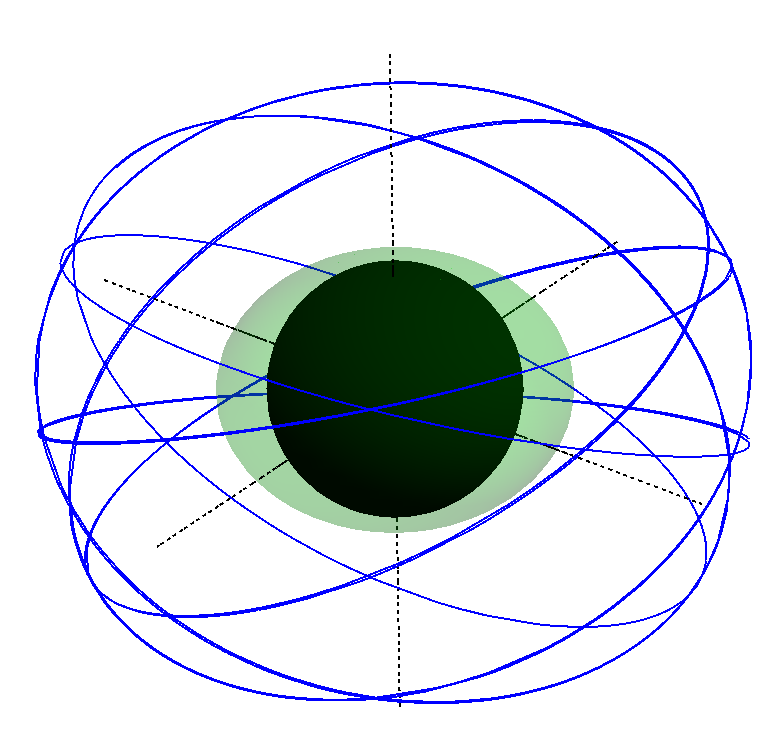
\includegraphics[width=0.7\textwidth]{img/Chapter4/ClosedOrbit.png}}
\end{tabular}
\caption{The figure shows a closed geodesic outside the outer horizon in the Kerr geometry. As is well known, closed geodesics are a very important class of orbits that provide very useful information of the spacetime and the geodesic taxonomy. In this figure, the closed orbit is not restricted to to any plane and runs across all the spacetime. }
\end{figure*}

\clearpage

\begin{figure*}
\centering
 \hspace*{-0.05\textwidth}
\begin{tabular}{cc}
\centerline{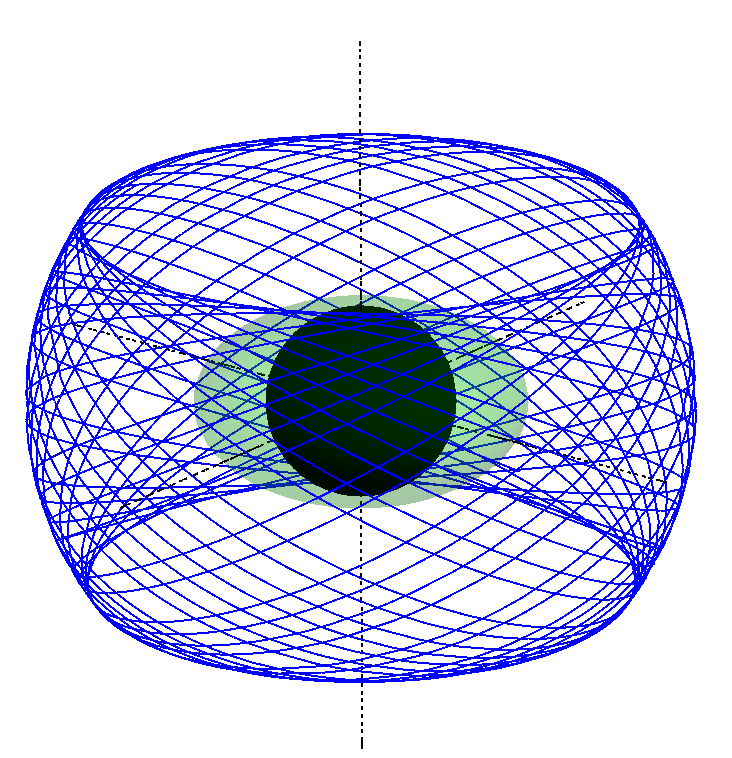
\includegraphics[width=0.7\textwidth]{img/Chapter4/Constantradius.png}}
\end{tabular}
\caption{The figure shows a geodesic with constant value of the coordinate $r$ (in \gls{BL} coordinates). This kind of motion is not as interesting as the closed orbit motion, but also provides useful information because, as we can see in the figure, this kind of geodesics are bounded between two limit circles whose height depend on the initial value of the Carter's constant. }
\end{figure*}

\clearpage

\begin{figure*}
\centering
 \hspace*{-0.05\textwidth}
\begin{tabular}{cc}
\centerline{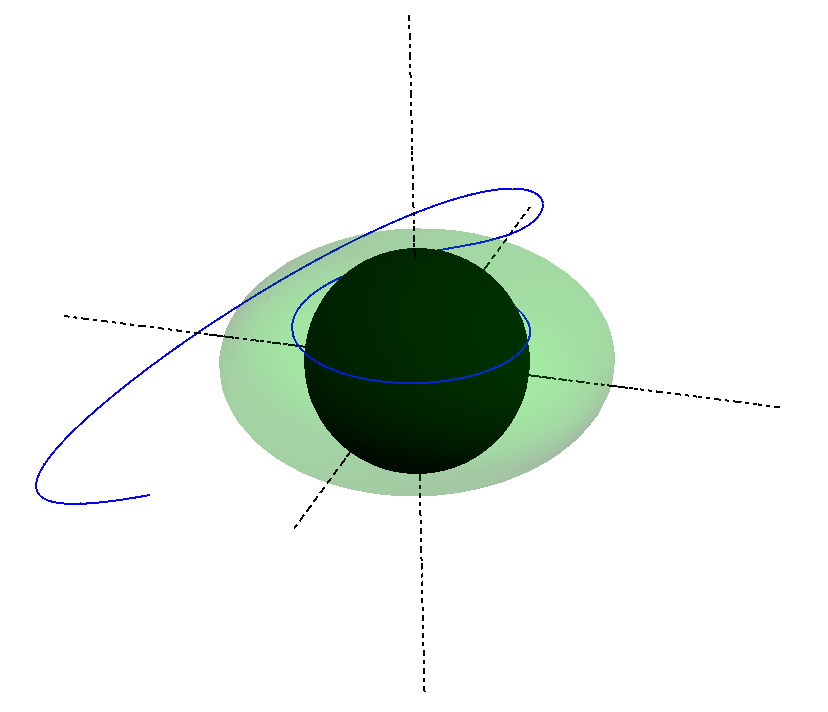
\includegraphics[width=1\textwidth]{img/Chapter4/Reversal.png}}
\end{tabular}
\caption{The figure shows what is known as the \textit{Ergosphere capture}, that is a process in which the geodesic tries to enter the ergosphere counterclockwise to the Kerr black hole rotation (in this case with its angular momentum pointing upwards) and as the properties of the Kerr geometry avoid that kind of movement, the geodesic is bend inwards and enters the ergosphere co-rotating with the Kerr black hole. Then, the geodesic is trapped in a circular co-rotating motion that ends in the outer horizon. This ergosphere capture is bounded to the equatorial plane.}
\end{figure*}

\clearpage

\begin{figure*}
\centering
 \hspace*{-0.05\textwidth}
\begin{tabular}{cc}
\centerline{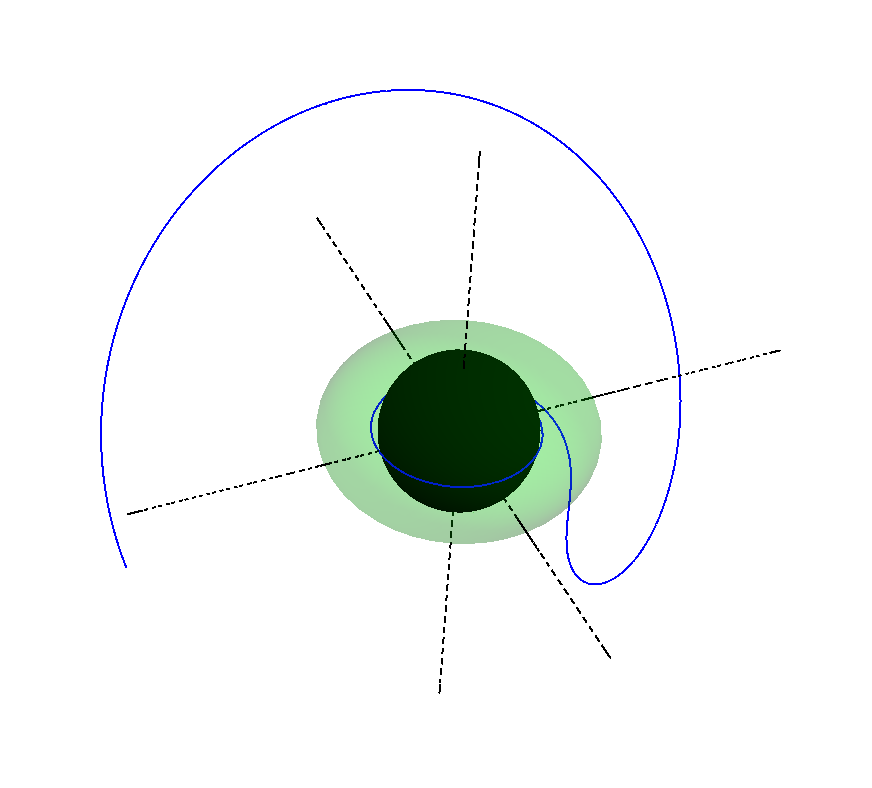
\includegraphics[width=1\textwidth]{img/Chapter4/Caputure.png}}
\end{tabular}
\caption{The figure shows another ergosphere capture but this time, the process is not bounded to a plane. As we can see in this image, the process is quite similar to the previous one, but this time the geodesic travels from the top to bottom after entering being captured by the ergosphere and bended inwards to be finally capture in a co-rotating movement that ends in the outer horizon.}
\end{figure*}


\clearpage


\begin{figure*}
\centering
\hspace*{-0.275\textwidth}
\begin{tabular}{cc}
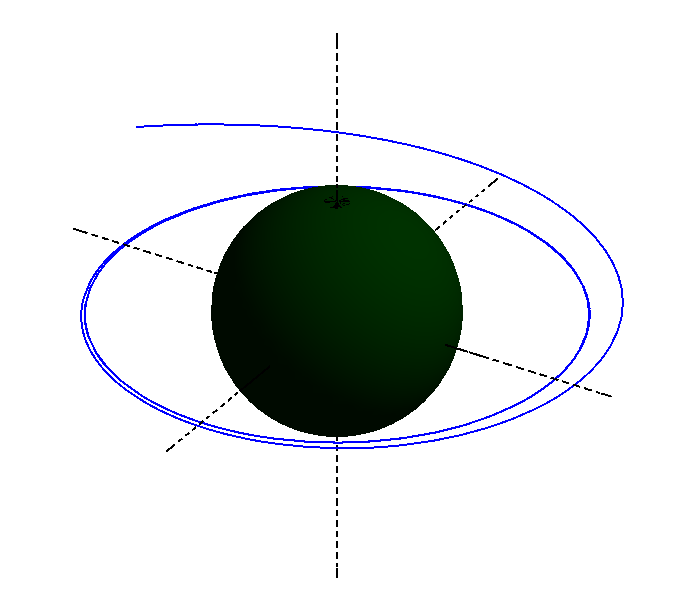
\includegraphics[width=0.6\textwidth]{img/Chapter4/ISCO1.png}&
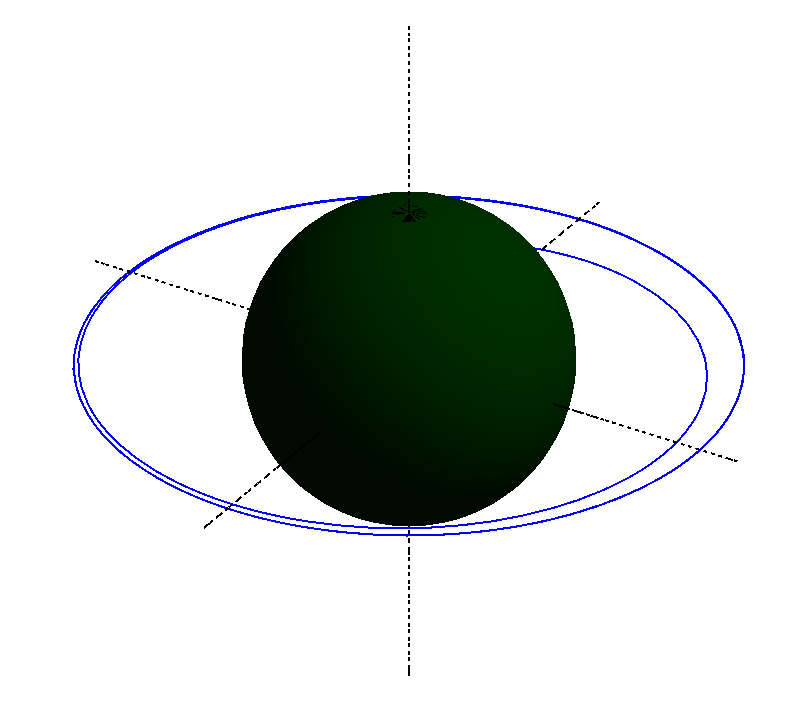
\includegraphics[width=0.6\textwidth]{img/Chapter4/ISCO2.png}\\
\end{tabular}
\caption{The two figures shows the behavior of the Innermost stable circular orbits (ISCOs). In the figure on the left, a geodesic that comes from the asymptotically flat region falls into the ISCO and remains there, while in the figure on the right, a particle that is initially at the ISCO is perturbed and trapped by the gravitational field of the black hole.}
\end{figure*}

\clearpage

\begin{figure*}
\centering
 \hspace*{-0.05\textwidth}
\centerline{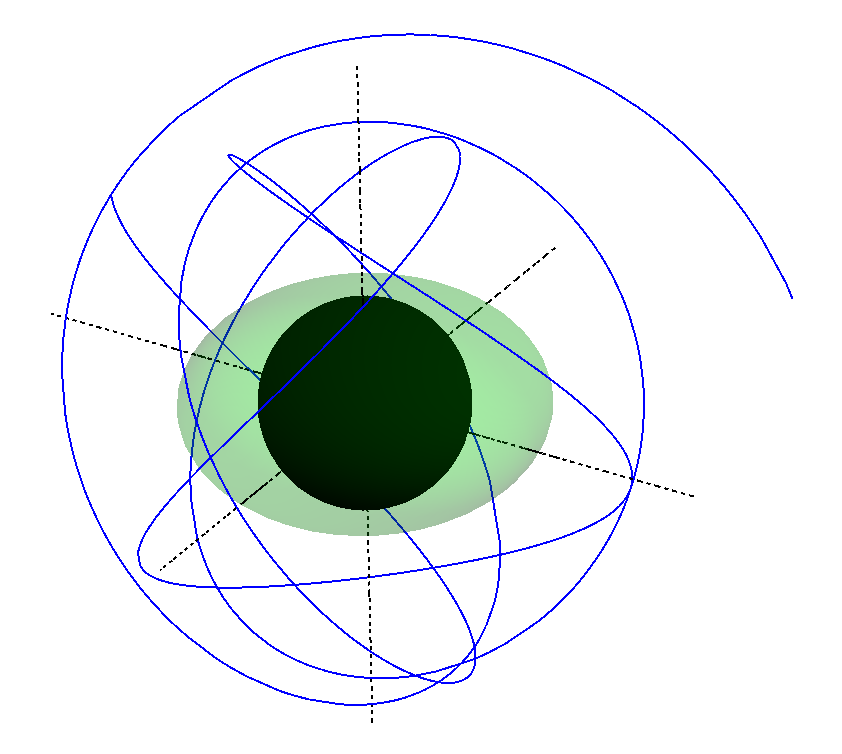
\includegraphics[width=1\textwidth]{img/Chapter4/Whirl.png}}
\caption{The figure shows what is known as the Whirl orbit. This kind of orbits may seem chaotic (and indeed they are) but they helped to understand and study the geodesic taxonomy based on the values of the Carter's constant. In this figure, the principal Whirl orbit is depicted. This kind of orbits are bounded asymptotically by the coordinate $r$ (in \gls{BL} coordinates) once they get near the ergosphere but they are not bounded by the coordinates $\theta$ and $\phi$, which gives the geodesic its characteristic behavior.}
\end{figure*}

\clearpage

\begin{figure*}
\centering
 \hspace*{-0.05\textwidth}
\centerline{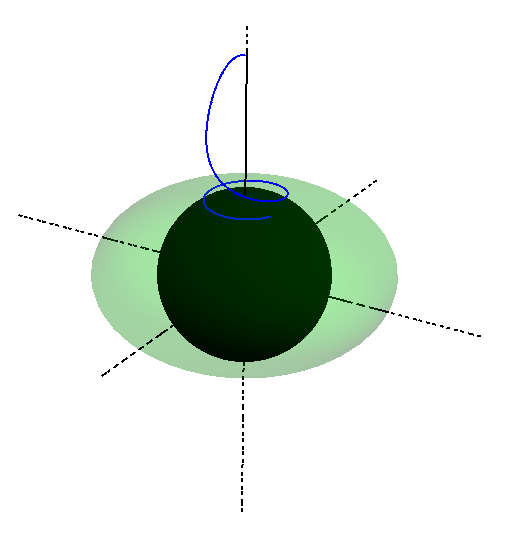
\includegraphics[width=0.75\textwidth]{img/Chapter4/ejein.png}}
\caption{The figure shows the real behavior of a geodesic trajectory that is perturbed away from the axis of symmetry. The geodesic go away from the axis and when reaches the ergosphere, the frame dragging effect starts and force the geodesic to spin co-rotating with the black hole to finally being captured by the outer horizon.}
\end{figure*}

\begin{figure*}
\centering
 \hspace*{-0.05\textwidth}
\centerline{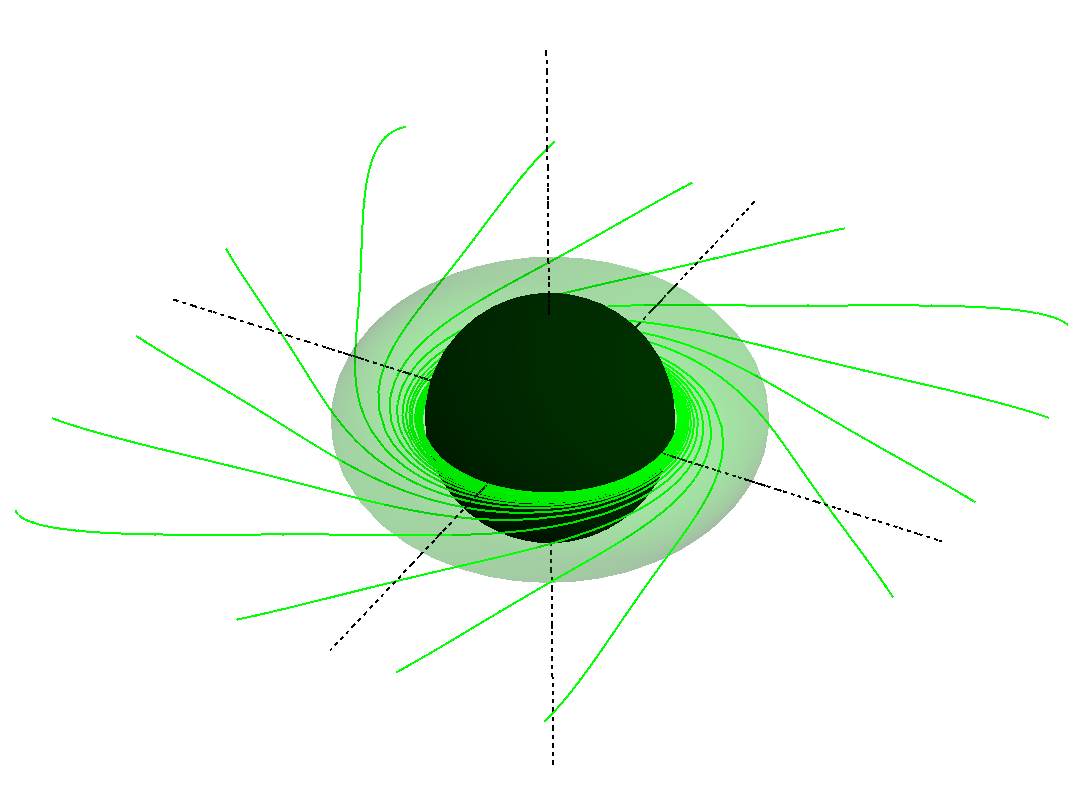
\includegraphics[width=0.85\textwidth]{img/Chapter4/ZAMOS.png}}
\caption{The figure shows the trajectories with zero angular momentum in the Kerr spacetime. Notice how in the first stages of the movement, the trajectories are straight lines and as the geodesics approaches the black hole, they are dragged by the ergosphere and acquire the \gls{ZAMO} angular velocity before cross the outer horizon.}
\end{figure*}



% 
% \begin{figure*}
% \centering
% \hspace*{-0.1\textwidth}
% \begin{tabular}{cc}
% 
% 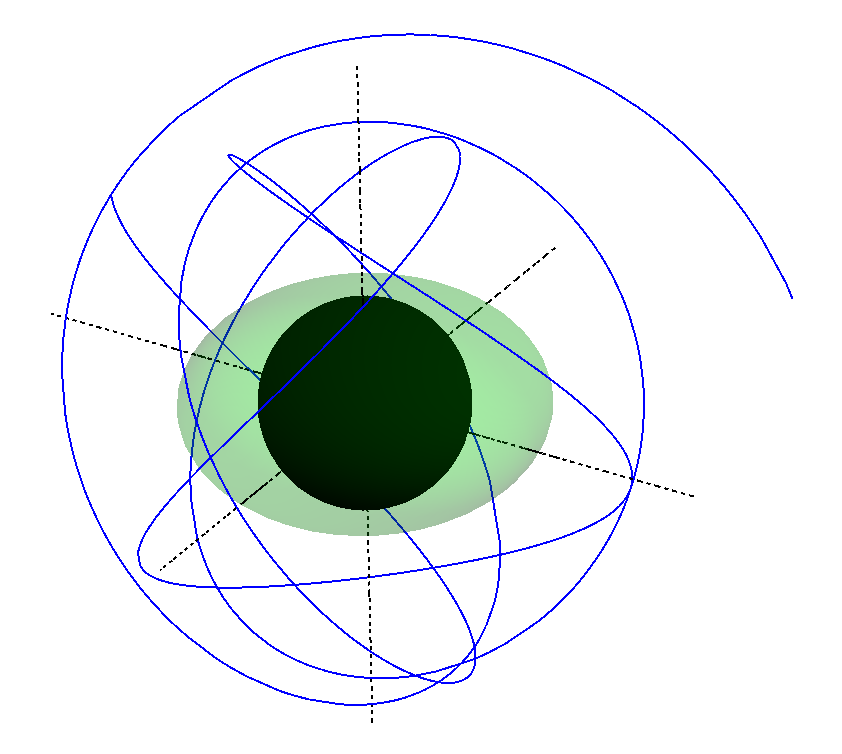
\includegraphics[width=0.5\textwidth]{img/Chapter4/Whirl.png}&
% 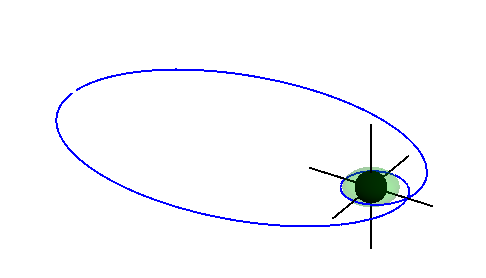
\includegraphics[width=0.5\textwidth]{img/Chapter4/Equatorial.png}\\
%
% \end{tabular}
% \end{figure*}